\paragraph{La classe Postman}

\begin{minipage}
    {\linewidth}
    \centering
    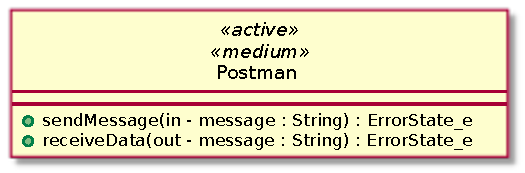
\includegraphics[width=0.50\linewidth]{../schemas/Conception_detaillee/classe_postman.pdf}
    \captionof{figure}{Diagramme de classe de Postman}
\end{minipage}

\subparagraph{Philosophie de conception \newline} 

\medspace

Postman est une classe qui permet de communiquer avec l'application {\nomApplication}. Elle échange divers messages avec l'application suivant le protocole de communication défini dans la \autoref{protocole_com}.

\subparagraph{Description structurelle \newline}

\medspace

\textbf{Attributs :}

N.A.

\textbf{Services offerts :}

\begin{itemize}
    \item \textbf{sendMessage(in - message : String) : ErrorState\_e} --- Opération qui permet d'envoyer un message à l'application {\nomApplication}.
    \item \textbf{receiveData(out - message : String) : ErrorState\_e} --- Opération qui permet de recevoir un message de l'application {\nomApplication}.
\end{itemize}
